% !TEX root = main.tex
% !TEX encoding = Windows Latin 1
% !TEX TS-program = pdflatex
% arara: pdflatexmk
%
% Plantilla para las tesis de ingenieria de la Universidad de los Andes
% 2012/07/27, v.1.9

% Para las opciones de clase, ver la documentacion
\documentclass[publish,english]{tui}
\checklanguage

%\include{personal} % Incluya aqui el archivo con su comandos personales y los paquetes adicionales que quiera cargar.

% !TEX root = main.tex
% !TEX encoding = Windows Latin 1
% !TEX TS-program = pdflatex
% 
% Archivo de particion de palabras

\hyphenation{%
  % Introduzca aqui las palabras que requieran division especial, separadas por espacios.
  % No se pueden usar acentos en estas palabras (a menos que se use codificacion UTF8).
  pa-la-bra guio-nes
  }


\endinput  % Excepciones de guiones (editar archivo)


% --------------------------------------------
% En caso de NO usar indice analitico (no recomendado),
% comentar esta seccion:
\makeatletter
  \iftui@draft\relax
    \else\makeindex % indice analitico
  \fi
\makeatother

%----------------------------------------------

\begin{document}% =========================================
\setupeverything
\frontmatter % Los preliminares de la tesis
\pagestyle{empty}

% !TEX root = main.tex
% !TEX encoding = Windows Latin 1
% !TEX TS-program = pdflatex
%
% portada.tex (portadilla y portada de la tesis)

% +++++++++++++++++++++++ Portadilla +++++++++++++++++++++++++++++
%
\pagestyle{empty}
\dosenblanco

% Portadilla
\begin{center}
  \scshape%
  % Aqui va el titulo de la tesis----------------------------------
  Este es el t\'{i}tulo \\
  de la tesis doctoral \\
  % ---------------------------------------------------------------
\end{center}

\cleardoublepage

% +++++++++++++++++++++++ Portada +++++++++++++++++++++++++++++
%
\begin{center}
{%
  \LARGE\scshape\bfseries%
  % Aqui va el titulo de la tesis ---------------------------
  Este es el t\'{i}tulo \\ [6pt]
  de la tesis doctoral \\ [6pt]
  % ---------------------------------------------------------
}

\vfill

{
 \large\scshape%
  A dissertation\\
  by\\
  % Aqui va el autor de la tesis-----------------------------
  Este es el autor de la tesis
  % ---------------------------------------------------------
}

\vfill

{%
  % Datos de la Universidad, el titulo, etc. ------------------
  {\normalfont Submitted to the School of Engineering of the}\\[3pt]
  {\large\scshape Universidad de los Andes}\\[3pt]
  {\normalfont in partial fulfillment for the requirements for the Degree of}\\[3pt]
  {\large\scshape Doctor in Engineering}
  % -------------------------------------------------------------
}

\vfill

%----------------------- No tocar este codigo ----------------------
\makeatletter
  \iftui@spanish
    {\scshape Aprobada por:}
  \else
    {\scshape Approved by:}
  \fi
\makeatother
% ------------------------------------------------------------------


% Llenar esta informacion ------------------------------------------
\begin{tabbing}
  \hspace{6.5cm}\=\kill
  \hspace{1cm}Committee Chair:    \> {\itshape Dr. . . . } \\
  \hspace{1cm}Committee Members:  \> {\itshape Prof. . . . } \\
  			    											 \> {\itshape Prof. . . . } \\
                                  \> {\itshape Prof. Dr. . . . } \\
                                  \> {\itshape Prof. Dr. . . . } \\
                                  \> {\itshape Prof. Dr. . . . } \\
                                  \> {\itshape Prof. Dr. . . . } \\
                                  \> {\itshape Prof. Dr. . . . } \\
                                  
  \hspace{1cm}Dean School of Engineering: \> {\itshape Dr. Alain Gauthier} \\
  \hspace{1cm}Assistant Dean: \> {\itshape Dr. Rubby Casallas}
\end{tabbing}
% --------------------------------------------------------------------

\vfill

{%
  \normalsize\scshape
  % Fecha y area --------------------------------------------------
  February 2011\\
  {\scshape%
  Field: Ingenier\'{i}a de Sistemas y Computaci\'{o}n
  % ---------------------------------------------------------------
  }
}

\end{center}



% Fin de portada.tex
\endinput  % Portadilla y portada (editar archivo)

\makeatletter
\iftui@publish
  % !TEX root = main.tex
% !TEX encoding = Windows Latin 1
% !TEX TS-program = pdflatex
%
% plegal.tex (Pagina legal de la tesis)


\hbox{}\thispagestyle{empty}

\vspace*{-2cm}
\begin{center}
\noindent
\fbox{\parbox{\textwidth}{%
\scriptsize
 \vspace*{3cm}

 [Informaci{\'o}n p{\'a}gina legal]

 \vspace*{3cm}
}}

\end{center}

\vfill


{%
\parindent=0pt
\scriptsize

Primera edici{\'o}n:  Febrero de 2010\\

\copyright\ [Nombre del autor]\\
\url{email@del.autor}

\medskip

\copyright\ Universidad de los Andes, Facultad de Ingenier\'{\i}a\\
\phantom{\copyright\ }Departamento de Ingenier\'{\i}a * * * * * * * * * * * * \\

\bigskip

Ediciones Uniandes\\ Carrera 1\textsuperscript{a} No. 19-27. Edificio AU 6\\
Bogot{\'a} \textsc{DC}, Colombia\\
Tel{\'e}fono: 339 49 49 / 339 49 99. Ext: 2133. Fax: ext. 2158\\
\url{http://ediciones.uniandes.edu.co/}\\
\url{infeduni@uniandes.edu.co}

\bigskip

ISBN: [N{\'u}mero del ISBN]

\bigskip

Correcci{\'o}n de estilo en ingl{\'e}s: xxxxxxxxxxxxxx

\bigskip

Dise{\~n}o de car{\'a}tula: xxxxxxxxxxxxxx

\bigskip

Dise{\~n}o de colecci{\'o}n: Nicol{\'a}s Vaughan

\bigskip

Impresi{\'o}n: [Nombre editorial] \\ \
[Direcci{\'o}n] \\ \
Bogot{\'a} \textsc{DC}, Colombia

}

\vfill

\begin{tiny}
\begin{flushleft}
\noindent  Impreso en Colombia -- Printed in Colombia\\

\noindent Todos los derechos reservados. Esta publicaci{\'o}n no puede
ser reproducida ni en su todo ni en sus partes, ni registrada en o
trasmitida por un sistema de recuperaci{\'o}n de informaci{\'o}n, en ninguna
forma ni por ning{\'u}n medio sea mec{\'a}nico, fotoqu\'{\i}mico, electr{\'o}nico,
magn{\'e}tico, electro-{\'o}ptico, por fotocopia o cualquier otro, sin el
permiso previo por escrito de la editorial.
\end{flushleft}
\end{tiny}

% Fin de plegal.tex
\endinput  % Pagina legal (editar archivo)
  % !TEX root = main.tex
% !TEX encoding = Windows Latin 1
% !TEX TS-program = pdflatex
%
% Archivo: coleccion.tex (Descripcion de la coleccion de tesis)

% ------------  Importante: No editar este archivo ----------------------------

\selectlanguage{spanish}
\chapter*{Descripci{\'o}n de la colecci{\'o}n}
\thispagestyle{empty}
\noindent
Esta colecci{\'o}n re{\'u}ne los mejores trabajos de grado de maestr\'{\i}a y de doctorado de la Facultad de Ingenier\'{\i}a de la Universidad de los Andes. Con el {\'a}nimo de divulgar estos resultados de nuestros grupos de investigaci{\'o}n, la Facultad los pone a disposici{\'o}n de la comunidad acad{\'e}mica.

\bigskip

\noindent
Decano, Alain Gauthier Sellier; Vicedecana de Posgrado e Investigaci{\'o}n, Rubby Casallas Guti{\'e}rrez; Vicedecano de Pregrado, Rafael G{\'o}mez D\'{\i}az; Vicedecano para el Sector Externo, Gonzalo Torres Cadena; Secretaria General, Claudia C{\'a}rdenas Guti{\'e}rrez; Directores de Departamento: de Ingenier\'{\i}a Civil y Ambiental, Arcesio Lizcano Pel{\'a}ez; de El{\'e}ctrica y Electr{\'o}nica, Roberto Bustamante Miller; de Industrial, Roberto Zarama Urdaneta; de Mec{\'a}ni\-ca, {\'E}dgar Alejandro Mara{\~n}{\'o}n Le{\'o}n; de Qu\'{\i}mica, {\'O}scar {\'A}lvarez Solano; de Sistemas y Computaci{\'o}n, Jorge Alberto Villalobos Salcedo.



\checklanguage
% Fin archivo coleccion.tex
\endinput 
 % Descripcion coleccion tesis (no editar archivo)
  \else\relax\fi
\makeatother

\cleardoublepage

% !TEX root = main.tex
% !TEX encoding = Windows Latin 1
% !TEX TS-program = pdflatex
% 
% agradec.tex (Agradecimientos de la tesis)

\thispagestyle{empty}

\ 

\vspace*{2cm}

{
\flushright\itshape

****,\\
****,\\
****.\\

}


\vfill




% Fin de dedicat.tex
\endinput  % Dedicatoria (opcional) (editar archivo)
% !TEX root = main.tex
% !TEX encoding = Windows Latin 1
% !TEX TS-program = pdflatex
% 
% agradec.tex (Agradecimientos de la tesis)

\Agradecimientos
\noindent








% Fin de agradec.tex
\endinput  % Agradecimientos (editar archivo)
This document gives a quick, relatively minimal example of the use of
\texttt{uafthesis.cls}, while trying to show its features.

This section is contained in \texttt{abstract.tex}.
 % Resumen ingles (editar archivo)
% !TEX root = main.tex
% !TEX encoding = Windows Latin 1
% !TEX TS-program = pdflatex
%
% Archivo: resumen.tex (en espanol)


\chapter{Resumen} % No cambiar el titulo
\selectlanguage{spanish}
\noindent
Duis tristique sollicitudin leo nec consequat. Praesent et dui convallis velit tincidunt fermentum. Mauris cursus purus at sem viverra sed imperdiet sapien imperdiet. Aliquam mattis, elit eget rutrum vulputate, tortor sem pulvinar justo, sit amet mollis felis sem at nibh. Donec malesuada, neque id interdum eleifend, arcu augue porta elit, nec tristique libero metus at massa. Fusce fringilla laoreet rhoncus. Suspendisse potenti. Phasellus dignissim sodales mauris at pharetra. Donec gravida fringilla velit ac rutrum.

Curabitur ornare lectus id diam molestie eu imperdiet nulla tempus. Maecenas vestibulum enim et dui ornare blandit. Vivamus fermentum faucibus viverra. Maecenas at justo sapien. Aenean rhoncus augue mattis purus rhoncus venenatis. Suspendisse metus felis, porttitor in varius in, vulputate at tortor. Aliquam molestie, turpis et malesuada porta, tortor sapien pharetra sapien, ac rhoncus quam dolor a sapien. Pellentesque varius laoreet enim ut auctor. Nullam nec ultricies nisi. Nullam porta lectus et ante consectetur posuere.


Curabitur ornare lectus id diam molestie eu imperdiet nulla tempus. Maecenas vestibulum enim et dui ornare blandit. Vivamus fermentum faucibus viverra. Maecenas at justo sapien. Aenean rhoncus augue mattis purus rhoncus venenatis. Suspendisse metus felis, porttitor in varius in, vulputate at tortor. Aliquam molestie, turpis et malesuada porta, tortor sapien pharetra sapien, ac rhoncus quam dolor a sapien. Pellentesque varius laoreet enim ut auctor. Nullam nec ultricies nisi. Nullam porta lectus et ante consectetur posuere.


\bigskip
\noindent
\textit{Palabras clave:} palabra uno; palabra dos; palabra tres.

\checklanguage
% Fin archivo resumen.tex
\endinput  % Resumen espanol (editar archivo)


% Tabla de contenido, dependiendo del idioma
\tuitableofcontents

\cleardoublepage

\listoftables  % En caso de que haya tablas --------------
% (comentar en caso contrario)

\cleardoublepage

\listoffigures % En caso de que haya figuras --------------
% (comentar en caso contrario)

\cleardoublepage

%% !TEX root = main.tex
% !TEX encoding = Windows Latin 1
% !TEX TS-program = pdflatex
% 
% Archivo: listofsymbols.tex (Lista de simbolos)


\ListofSymbols
\ 
% ------------- Editar tabla -----------------------
\begin{center}
\begin{tabular}{rl}
  $\wedge$ & and \\
  $\vee$ & or \\
  $\rightarrow$ & material conditional \\
  $\leftrightarrow$ & material biconditional \\
  $\vdash$ & logical derivability \\
  $\neg$ & negation\\
  $\forall$ & universal quantification\\
  $\exists$ & existential quantification\\
  $\top$ & true\\
  $\bot$ & false\\
  $\Box$ & necessity\\
  $\diamond$ & contingency\\
\end{tabular}
\end{center}

% ----------------------------------------------------


% Fin archivo listofsymbols.tex
\endinput % (editar archivo)--------------
% (comentar si no es usado)

\cleardoublepage

\section{Introduction}
\label{sec:introduction}

To accompany \TeX{}, Knuth developed \MF{} as a method of ``creating
entire families of fonts from a set of dimensional parameters and
outline descriptions''~\cite{beebe:mf}.  Approximately ten years later,
John Hobby began work on \MP{}\Dash ``a powerful graphics language based
on Knuth's \MF, but with PostScript output and facilities for including
typeset text''~\cite{hobby:user}.  Although several packages (e.g.,
\PiC\TeX, \Xy-pic, and the native \LaTeX{} picture environment to name a
few) are available for creating graphics within \TeX-based documents,
they all rely on \TeX{}.  Since \TeX{} was designed to typeset text, it
seems natural that an external utility should be used to generate
graphics instead.  Furthermore, in the event that the graphics require
typeset text, then the utility should use \TeX{} for this requirement.
This premise is exactly the philosophy of \MP.

Since \MP{} is a programming language, it accommodates data structures
and flow control, and compilation of the \MP{} source code yields \EPS{}
graphics.  These features provide an elegant method for generating
graphics.  \autoref{fig:circles} illustrates how \MP{} can be used
programatically.  The figure is generated by rotating one of the circles
multiple times to obtain the desired \textit{circular chain}.%
\footnote{All graphics in this tutorial (except \autoref{fig:previewer})
  are created with \MP{}, and the source code and any required external
  data files for each of these graphics are embedded as file attachments
  in the electronic \PDF{} version of the article.  Attachments are
  indicated by a paper clip icon.

  \vspace{-\baselineskip}
  \noindent%
  \raisebox{0pt}[0pt][0pt]{%
    \makebox[0pt][r]{%
      \notextattachfile{\paperclip}%
      \hspace*{\marginparsep}%
    }%
  }%
}

\begin{figure}
  \begin{withattachment}{circles.mp}
    \centering
    \includegraphics{circles.mps}
  \end{withattachment}
  \caption{Rotated circles}
  \label{fig:circles}
\end{figure}

The programming language constructs of \MP{} also deliver a graceful
mechanism for creating animations without having to manually create each
frame of the animation.  The primary advantage of \EPS{} is that it can
be scaled to any resolution without a loss in quality.  It can also be
easily converted to raster formats, e.g.\ Portable Network Graphics
(\PNG) and Joint Photographic Experts Group (\JPEG), et al., or other
vector formats including Portable Document Format (\PDF) and Scalable
Vector Graphics (\SVG), et al.
 % Introduccion de la tesis (editar archivo)

% -----------------------------------------------------------
\mainmatter % Cuerpo de la tesis
\pagestyle{tui}

\chapter{Introduction} \label{cha:intro}
Here is some introductory text regarding the thesis.
Ideally, the introduction should be longer than one page. 
This way, the reader will have some vague idea of what it is that you'll be presenting.

I have added liberal blind text here to extend this chapter onto a second page.  
We can then check the pagination and other important things. 
This chapter should be introducing the topic of your thesis and providing motivation to your work.

Figure~\ref{fig:test2} shows a sample figure. More details are discussed in Appendix~\ref{app:test}.
\begin{figure}
  \centering 
  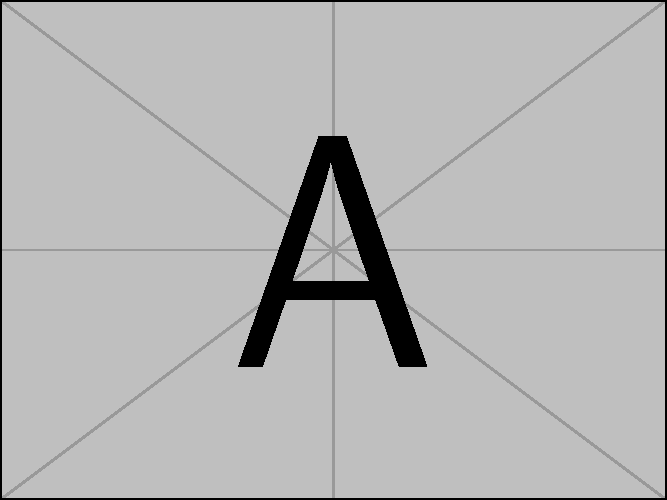
\includegraphics[width=1in]{example-image-a}
  \caption{This test figure tests captions and Table of Contents 
    behavior for very lengthy captions.}
  \label{fig:test2}
\end{figure}

\section{Background}
Test sectioning commands.  We can also have \verb+subsection+, \verb+subsubsection+,
\verb+paragraph+, and \verb+subparagraph+.  Let's try a few:

\subsection{Test Subsection}
\lipsum[1]

\subsection{Another Subsection}
Testing display mathematics:
\begin{equation}
e = mc^2,
\end{equation}
where $e$ is the energy, $m$ is the mass, and the constant $c$ represents the speed of light in a vacuum.

\subsubsection{Subheading}
\lipsum[3-5]
 % Capitulo 1 (editar archivo)
\chapter{Literature Review} \label{cha:litreview}
As you can see here, the author has performed an exhaustive literature review to provide
a solid foundation on which the remainder of this thesis is built.
\begin{quote}
This is a test of the \verb+quote+ environment. We should be in single-spaced mode and with some additional indentation to set this off from the rest of the text.
\end{quote}
Now we should have returned to double-spaced mode and regular indentation/margins.
Let's add some more text here to fill the page and check the glue settings.
We need more text on this page for testing purposes.

Now let's test the \verb+quotation+ environment:
\begin{quotation}
This is a test of the \verb+quotation+ environment. We should be in single-spaced mode and with some additional indentation to set this off from the rest of the text.
\end{quotation}
Here we return%
\footnote{
  This is a test footnote extending over more than one line. 
  This should be in single-spaced mode according to the MUGS Thesis Directives.
} 
to normal text mode.

\lipsum % Capitulo 2 (editar archivo)
% !TEX root = main.tex
% !TEX encoding = Windows Latin 1
% !TEX TS-program = pdflatex
% 
% Archivo: ch03.tex (Capitulo 3)

\chapter{*******}
\section{*******}




% Fin archivo ch03.tex
\endinput  % Capitulo 3 (editar archivo)
%\include{ch04} % etc...
% Anadir los que sean necesarios.

\appendix % Apendices de la tesis
% !TEX root = main.tex
% !TEX encoding = Windows Latin 1
% !TEX TS-program = pdflatex
% 
% Archivo: ap01.tex (Apendice 1)

\chapter{This Is My First Appendix bla bla bla bla bla bla bla bla}
\section{This Is My First Section bla bla bla bla bla bla bla bla bla bla bla bla }
\noindent
First sentence.\footnote{And this is my first footnote. And this is my first footnote. And this is my first footnote. And this is my first footnote. And this is my first footnote. And this is my first footnote. And this is my first footnote. And this is my first footnote. And this is my first footnote. And this is my first footnote. And this is my first footnote. And this is my first footnote. And this is my first footnote. And this is my first footnote. And this is my first footnote.}\index{Concepto}

\subsection{This Is My First Subsection}
\noindent
% !TEX root = main.tex
% !TEX encoding = Windows Latin 1
% !TEX TS-program = pdflatex
% 
Duis tristique \index{sollicitudin} sollicitudin leo nec consequat. Praesent et dui convallis velit tincidunt fermentum. Mauris cursus purus at sem viverra sed imperdiet sapien imperdiet. Aliquam mattis, elit eget rutrum vulputate, tortor sem pulvinar justo, sit amet mollis felis sem at nibh. Donec malesuada, neque id interdum eleifend, arcu augue porta elit, nec tristique libero metus at massa. Fusce fringilla laoreet rhoncus. Suspendisse potenti. Phasellus dignissim sodales mauris at pharetra. Donec gravida fringilla velit ac rutrum. Curabitur ornare lectus id diam molestie eu imperdiet nulla tempus. Maecenas vestibulum enim et dui ornare blandit. Vivamus \index{fermentum} faucibus viverra. Maecenas at justo sapien. Aenean rhoncus augue mattis purus rhoncus venenatis. Suspendisse metus felis, porttitor in varius in, vulputate at tortor. Aliquam molestie, turpis et malesuada porta, tortor sapien pharetra sapien, ac rhoncus quam dolor a sapien. Pellentesque varius laoreet enim ut auctor. Nullam nec ultricies nisi. Nullam porta lectus et ante consectetur posuere. \cite{texbook} 

% !TEX root = main.tex
% !TEX encoding = Windows Latin 1
% !TEX TS-program = pdflatex
% 
Duis tristique \index{sollicitudin} sollicitudin leo nec consequat. Praesent et dui convallis velit tincidunt fermentum. Mauris cursus purus at sem viverra sed imperdiet sapien imperdiet. Aliquam mattis, elit eget rutrum vulputate, tortor sem pulvinar justo, sit amet mollis felis sem at nibh. Donec malesuada, neque id interdum eleifend, arcu augue porta elit, nec tristique libero metus at massa. Fusce fringilla laoreet rhoncus. Suspendisse potenti. Phasellus dignissim sodales mauris at pharetra. Donec gravida fringilla velit ac rutrum. Curabitur ornare lectus id diam molestie eu imperdiet nulla tempus. Maecenas vestibulum enim et dui ornare blandit. Vivamus \index{fermentum} faucibus viverra. Maecenas at justo sapien. Aenean rhoncus augue mattis purus rhoncus venenatis. Suspendisse metus felis, porttitor in varius in, vulputate at tortor. Aliquam molestie, turpis et malesuada porta, tortor sapien pharetra sapien, ac rhoncus quam dolor a sapien. Pellentesque varius laoreet enim ut auctor. Nullam nec ultricies nisi. Nullam porta lectus et ante consectetur posuere. 

% !TEX root = main.tex
% !TEX encoding = Windows Latin 1
% !TEX TS-program = pdflatex
% 
Duis tristique \index{sollicitudin} sollicitudin leo nec consequat. Praesent et dui convallis velit tincidunt fermentum. Mauris cursus purus at sem viverra sed imperdiet sapien imperdiet. Aliquam mattis, elit eget rutrum vulputate, tortor sem pulvinar justo, sit amet mollis felis sem at nibh. Donec malesuada, neque id interdum eleifend, arcu augue porta elit, nec tristique libero metus at massa. Fusce fringilla laoreet rhoncus. Suspendisse potenti. Phasellus dignissim sodales mauris at pharetra. Donec gravida fringilla velit ac rutrum. Curabitur ornare lectus id diam molestie eu imperdiet nulla tempus. Maecenas vestibulum enim et dui ornare blandit. Vivamus \index{fermentum} faucibus viverra. Maecenas at justo sapien. Aenean rhoncus augue mattis purus rhoncus venenatis. Suspendisse metus felis, porttitor in varius in, vulputate at tortor. Aliquam molestie, turpis et malesuada porta, tortor sapien pharetra sapien, ac rhoncus quam dolor a sapien. Pellentesque varius laoreet enim ut auctor. Nullam nec ultricies nisi. Nullam porta lectus et ante consectetur posuere. 

% !TEX root = main.tex
% !TEX encoding = Windows Latin 1
% !TEX TS-program = pdflatex
% 
Duis tristique \index{sollicitudin} sollicitudin leo nec consequat. Praesent et dui convallis velit tincidunt fermentum. Mauris cursus purus at sem viverra sed imperdiet sapien imperdiet. Aliquam mattis, elit eget rutrum vulputate, tortor sem pulvinar justo, sit amet mollis felis sem at nibh. Donec malesuada, neque id interdum eleifend, arcu augue porta elit, nec tristique libero metus at massa. Fusce fringilla laoreet rhoncus. Suspendisse potenti. Phasellus dignissim sodales mauris at pharetra. Donec gravida fringilla velit ac rutrum. Curabitur ornare lectus id diam molestie eu imperdiet nulla tempus. Maecenas vestibulum enim et dui ornare blandit. Vivamus \index{fermentum} faucibus viverra. Maecenas at justo sapien. Aenean rhoncus augue mattis purus rhoncus venenatis. Suspendisse metus felis, porttitor in varius in, vulputate at tortor. Aliquam molestie, turpis et malesuada porta, tortor sapien pharetra sapien, ac rhoncus quam dolor a sapien. Pellentesque varius laoreet enim ut auctor. Nullam nec ultricies nisi. Nullam porta lectus et ante consectetur posuere. 

\subsubsection{This Is My First Subsubsection}
\noindent
% !TEX root = main.tex
% !TEX encoding = Windows Latin 1
% !TEX TS-program = pdflatex
% 
Duis tristique \index{sollicitudin} sollicitudin leo nec consequat. Praesent et dui convallis velit tincidunt fermentum. Mauris cursus purus at sem viverra sed imperdiet sapien imperdiet. Aliquam mattis, elit eget rutrum vulputate, tortor sem pulvinar justo, sit amet mollis felis sem at nibh. Donec malesuada, neque id interdum eleifend, arcu augue porta elit, nec tristique libero metus at massa. Fusce fringilla laoreet rhoncus. Suspendisse potenti. Phasellus dignissim sodales mauris at pharetra. Donec gravida fringilla velit ac rutrum. Curabitur ornare lectus id diam molestie eu imperdiet nulla tempus. Maecenas vestibulum enim et dui ornare blandit. Vivamus \index{fermentum} faucibus viverra. Maecenas at justo sapien. Aenean rhoncus augue mattis purus rhoncus venenatis. Suspendisse metus felis, porttitor in varius in, vulputate at tortor. Aliquam molestie, turpis et malesuada porta, tortor sapien pharetra sapien, ac rhoncus quam dolor a sapien. Pellentesque varius laoreet enim ut auctor. Nullam nec ultricies nisi. Nullam porta lectus et ante consectetur posuere. \cite{texbook}

% !TEX root = main.tex
% !TEX encoding = Windows Latin 1
% !TEX TS-program = pdflatex
% 
Duis tristique \index{sollicitudin} sollicitudin leo nec consequat. Praesent et dui convallis velit tincidunt fermentum. Mauris cursus purus at sem viverra sed imperdiet sapien imperdiet. Aliquam mattis, elit eget rutrum vulputate, tortor sem pulvinar justo, sit amet mollis felis sem at nibh. Donec malesuada, neque id interdum eleifend, arcu augue porta elit, nec tristique libero metus at massa. Fusce fringilla laoreet rhoncus. Suspendisse potenti. Phasellus dignissim sodales mauris at pharetra. Donec gravida fringilla velit ac rutrum. Curabitur ornare lectus id diam molestie eu imperdiet nulla tempus. Maecenas vestibulum enim et dui ornare blandit. Vivamus \index{fermentum} faucibus viverra. Maecenas at justo sapien. Aenean rhoncus augue mattis purus rhoncus venenatis. Suspendisse metus felis, porttitor in varius in, vulputate at tortor. Aliquam molestie, turpis et malesuada porta, tortor sapien pharetra sapien, ac rhoncus quam dolor a sapien. Pellentesque varius laoreet enim ut auctor. Nullam nec ultricies nisi. Nullam porta lectus et ante consectetur posuere. 

% !TEX root = main.tex
% !TEX encoding = Windows Latin 1
% !TEX TS-program = pdflatex
% 
Duis tristique \index{sollicitudin} sollicitudin leo nec consequat. Praesent et dui convallis velit tincidunt fermentum. Mauris cursus purus at sem viverra sed imperdiet sapien imperdiet. Aliquam mattis, elit eget rutrum vulputate, tortor sem pulvinar justo, sit amet mollis felis sem at nibh. Donec malesuada, neque id interdum eleifend, arcu augue porta elit, nec tristique libero metus at massa. Fusce fringilla laoreet rhoncus. Suspendisse potenti. Phasellus dignissim sodales mauris at pharetra. Donec gravida fringilla velit ac rutrum. Curabitur ornare lectus id diam molestie eu imperdiet nulla tempus. Maecenas vestibulum enim et dui ornare blandit. Vivamus \index{fermentum} faucibus viverra. Maecenas at justo sapien. Aenean rhoncus augue mattis purus rhoncus venenatis. Suspendisse metus felis, porttitor in varius in, vulputate at tortor. Aliquam molestie, turpis et malesuada porta, tortor sapien pharetra sapien, ac rhoncus quam dolor a sapien. Pellentesque varius laoreet enim ut auctor. Nullam nec ultricies nisi. Nullam porta lectus et ante consectetur posuere. 

% !TEX root = main.tex
% !TEX encoding = Windows Latin 1
% !TEX TS-program = pdflatex
% 
Duis tristique \index{sollicitudin} sollicitudin leo nec consequat. Praesent et dui convallis velit tincidunt fermentum. Mauris cursus purus at sem viverra sed imperdiet sapien imperdiet. Aliquam mattis, elit eget rutrum vulputate, tortor sem pulvinar justo, sit amet mollis felis sem at nibh. Donec malesuada, neque id interdum eleifend, arcu augue porta elit, nec tristique libero metus at massa. Fusce fringilla laoreet rhoncus. Suspendisse potenti. Phasellus dignissim sodales mauris at pharetra. Donec gravida fringilla velit ac rutrum. Curabitur ornare lectus id diam molestie eu imperdiet nulla tempus. Maecenas vestibulum enim et dui ornare blandit. Vivamus \index{fermentum} faucibus viverra. Maecenas at justo sapien. Aenean rhoncus augue mattis purus rhoncus venenatis. Suspendisse metus felis, porttitor in varius in, vulputate at tortor. Aliquam molestie, turpis et malesuada porta, tortor sapien pharetra sapien, ac rhoncus quam dolor a sapien. Pellentesque varius laoreet enim ut auctor. Nullam nec ultricies nisi. Nullam porta lectus et ante consectetur posuere. 

\section{This Is My Second Section}
\noindent
% !TEX root = main.tex
% !TEX encoding = Windows Latin 1
% !TEX TS-program = pdflatex
% 
Duis tristique \index{sollicitudin} sollicitudin leo nec consequat. Praesent et dui convallis velit tincidunt fermentum. Mauris cursus purus at sem viverra sed imperdiet sapien imperdiet. Aliquam mattis, elit eget rutrum vulputate, tortor sem pulvinar justo, sit amet mollis felis sem at nibh. Donec malesuada, neque id interdum eleifend, arcu augue porta elit, nec tristique libero metus at massa. Fusce fringilla laoreet rhoncus. Suspendisse potenti. Phasellus dignissim sodales mauris at pharetra. Donec gravida fringilla velit ac rutrum. Curabitur ornare lectus id diam molestie eu imperdiet nulla tempus. Maecenas vestibulum enim et dui ornare blandit. Vivamus \index{fermentum} faucibus viverra. Maecenas at justo sapien. Aenean rhoncus augue mattis purus rhoncus venenatis. Suspendisse metus felis, porttitor in varius in, vulputate at tortor. Aliquam molestie, turpis et malesuada porta, tortor sapien pharetra sapien, ac rhoncus quam dolor a sapien. Pellentesque varius laoreet enim ut auctor. Nullam nec ultricies nisi. Nullam porta lectus et ante consectetur posuere. \footnote{See also \cite{Aup91,Dou72,Hal82}.}


% !TEX root = main.tex
% !TEX encoding = Windows Latin 1
% !TEX TS-program = pdflatex
% 
Duis tristique \index{sollicitudin} sollicitudin leo nec consequat. Praesent et dui convallis velit tincidunt fermentum. Mauris cursus purus at sem viverra sed imperdiet sapien imperdiet. Aliquam mattis, elit eget rutrum vulputate, tortor sem pulvinar justo, sit amet mollis felis sem at nibh. Donec malesuada, neque id interdum eleifend, arcu augue porta elit, nec tristique libero metus at massa. Fusce fringilla laoreet rhoncus. Suspendisse potenti. Phasellus dignissim sodales mauris at pharetra. Donec gravida fringilla velit ac rutrum. Curabitur ornare lectus id diam molestie eu imperdiet nulla tempus. Maecenas vestibulum enim et dui ornare blandit. Vivamus \index{fermentum} faucibus viverra. Maecenas at justo sapien. Aenean rhoncus augue mattis purus rhoncus venenatis. Suspendisse metus felis, porttitor in varius in, vulputate at tortor. Aliquam molestie, turpis et malesuada porta, tortor sapien pharetra sapien, ac rhoncus quam dolor a sapien. Pellentesque varius laoreet enim ut auctor. Nullam nec ultricies nisi. Nullam porta lectus et ante consectetur posuere. 

% !TEX root = main.tex
% !TEX encoding = Windows Latin 1
% !TEX TS-program = pdflatex
% 
Duis tristique \index{sollicitudin} sollicitudin leo nec consequat. Praesent et dui convallis velit tincidunt fermentum. Mauris cursus purus at sem viverra sed imperdiet sapien imperdiet. Aliquam mattis, elit eget rutrum vulputate, tortor sem pulvinar justo, sit amet mollis felis sem at nibh. Donec malesuada, neque id interdum eleifend, arcu augue porta elit, nec tristique libero metus at massa. Fusce fringilla laoreet rhoncus. Suspendisse potenti. Phasellus dignissim sodales mauris at pharetra. Donec gravida fringilla velit ac rutrum. Curabitur ornare lectus id diam molestie eu imperdiet nulla tempus. Maecenas vestibulum enim et dui ornare blandit. Vivamus \index{fermentum} faucibus viverra. Maecenas at justo sapien. Aenean rhoncus augue mattis purus rhoncus venenatis. Suspendisse metus felis, porttitor in varius in, vulputate at tortor. Aliquam molestie, turpis et malesuada porta, tortor sapien pharetra sapien, ac rhoncus quam dolor a sapien. Pellentesque varius laoreet enim ut auctor. Nullam nec ultricies nisi. Nullam porta lectus et ante consectetur posuere. 

% !TEX root = main.tex
% !TEX encoding = Windows Latin 1
% !TEX TS-program = pdflatex
% 
Duis tristique \index{sollicitudin} sollicitudin leo nec consequat. Praesent et dui convallis velit tincidunt fermentum. Mauris cursus purus at sem viverra sed imperdiet sapien imperdiet. Aliquam mattis, elit eget rutrum vulputate, tortor sem pulvinar justo, sit amet mollis felis sem at nibh. Donec malesuada, neque id interdum eleifend, arcu augue porta elit, nec tristique libero metus at massa. Fusce fringilla laoreet rhoncus. Suspendisse potenti. Phasellus dignissim sodales mauris at pharetra. Donec gravida fringilla velit ac rutrum. Curabitur ornare lectus id diam molestie eu imperdiet nulla tempus. Maecenas vestibulum enim et dui ornare blandit. Vivamus \index{fermentum} faucibus viverra. Maecenas at justo sapien. Aenean rhoncus augue mattis purus rhoncus venenatis. Suspendisse metus felis, porttitor in varius in, vulputate at tortor. Aliquam molestie, turpis et malesuada porta, tortor sapien pharetra sapien, ac rhoncus quam dolor a sapien. Pellentesque varius laoreet enim ut auctor. Nullam nec ultricies nisi. Nullam porta lectus et ante consectetur posuere. 

\begin{table}[h]
  \begin{center}
\begin{tabular}{|r|l|}
  \hline
  7C0 & hexadecimal \\
  3700 & octal \\ \cline{2-2}
  11111000000 & binary \\
  \hline \hline
  1984 & decimal \\
  \hline
\end{tabular}
\caption{This is my first table}
\end{center}
\end{table}

\section{This Is My Third Section}
\noindent
% !TEX root = main.tex
% !TEX encoding = Windows Latin 1
% !TEX TS-program = pdflatex
% 
Duis tristique \index{sollicitudin} sollicitudin leo nec consequat. Praesent et dui convallis velit tincidunt fermentum. Mauris cursus purus at sem viverra sed imperdiet sapien imperdiet. Aliquam mattis, elit eget rutrum vulputate, tortor sem pulvinar justo, sit amet mollis felis sem at nibh. Donec malesuada, neque id interdum eleifend, arcu augue porta elit, nec tristique libero metus at massa. Fusce fringilla laoreet rhoncus. Suspendisse potenti. Phasellus dignissim sodales mauris at pharetra. Donec gravida fringilla velit ac rutrum. Curabitur ornare lectus id diam molestie eu imperdiet nulla tempus. Maecenas vestibulum enim et dui ornare blandit. Vivamus \index{fermentum} faucibus viverra. Maecenas at justo sapien. Aenean rhoncus augue mattis purus rhoncus venenatis. Suspendisse metus felis, porttitor in varius in, vulputate at tortor. Aliquam molestie, turpis et malesuada porta, tortor sapien pharetra sapien, ac rhoncus quam dolor a sapien. Pellentesque varius laoreet enim ut auctor. Nullam nec ultricies nisi. Nullam porta lectus et ante consectetur posuere. 
\begin{figure}[h]
  \begin{center}
    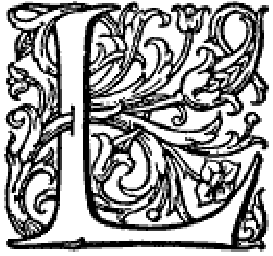
\includegraphics{imagen}
    \caption{This is my first figure}
  \end{center}
\end{figure}


% !TEX root = main.tex
% !TEX encoding = Windows Latin 1
% !TEX TS-program = pdflatex
% 
Duis tristique \index{sollicitudin} sollicitudin leo nec consequat. Praesent et dui convallis velit tincidunt fermentum. Mauris cursus purus at sem viverra sed imperdiet sapien imperdiet. Aliquam mattis, elit eget rutrum vulputate, tortor sem pulvinar justo, sit amet mollis felis sem at nibh. Donec malesuada, neque id interdum eleifend, arcu augue porta elit, nec tristique libero metus at massa. Fusce fringilla laoreet rhoncus. Suspendisse potenti. Phasellus dignissim sodales mauris at pharetra. Donec gravida fringilla velit ac rutrum. Curabitur ornare lectus id diam molestie eu imperdiet nulla tempus. Maecenas vestibulum enim et dui ornare blandit. Vivamus \index{fermentum} faucibus viverra. Maecenas at justo sapien. Aenean rhoncus augue mattis purus rhoncus venenatis. Suspendisse metus felis, porttitor in varius in, vulputate at tortor. Aliquam molestie, turpis et malesuada porta, tortor sapien pharetra sapien, ac rhoncus quam dolor a sapien. Pellentesque varius laoreet enim ut auctor. Nullam nec ultricies nisi. Nullam porta lectus et ante consectetur posuere. 

\begin{figure}[h]
  \begin{center}
    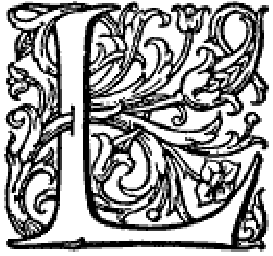
\includegraphics{imagen}
    \caption{This is my second figure}
  \end{center}
\end{figure}

% !TEX root = main.tex
% !TEX encoding = Windows Latin 1
% !TEX TS-program = pdflatex
% 
Duis tristique \index{sollicitudin} sollicitudin leo nec consequat. Praesent et dui convallis velit tincidunt fermentum. Mauris cursus purus at sem viverra sed imperdiet sapien imperdiet. Aliquam mattis, elit eget rutrum vulputate, tortor sem pulvinar justo, sit amet mollis felis sem at nibh. Donec malesuada, neque id interdum eleifend, arcu augue porta elit, nec tristique libero metus at massa. Fusce fringilla laoreet rhoncus. Suspendisse potenti. Phasellus dignissim sodales mauris at pharetra. Donec gravida fringilla velit ac rutrum. Curabitur ornare lectus id diam molestie eu imperdiet nulla tempus. Maecenas vestibulum enim et dui ornare blandit. Vivamus \index{fermentum} faucibus viverra. Maecenas at justo sapien. Aenean rhoncus augue mattis purus rhoncus venenatis. Suspendisse metus felis, porttitor in varius in, vulputate at tortor. Aliquam molestie, turpis et malesuada porta, tortor sapien pharetra sapien, ac rhoncus quam dolor a sapien. Pellentesque varius laoreet enim ut auctor. Nullam nec ultricies nisi. Nullam porta lectus et ante consectetur posuere. 

% !TEX root = main.tex
% !TEX encoding = Windows Latin 1
% !TEX TS-program = pdflatex
% 
Duis tristique \index{sollicitudin} sollicitudin leo nec consequat. Praesent et dui convallis velit tincidunt fermentum. Mauris cursus purus at sem viverra sed imperdiet sapien imperdiet. Aliquam mattis, elit eget rutrum vulputate, tortor sem pulvinar justo, sit amet mollis felis sem at nibh. Donec malesuada, neque id interdum eleifend, arcu augue porta elit, nec tristique libero metus at massa. Fusce fringilla laoreet rhoncus. Suspendisse potenti. Phasellus dignissim sodales mauris at pharetra. Donec gravida fringilla velit ac rutrum. Curabitur ornare lectus id diam molestie eu imperdiet nulla tempus. Maecenas vestibulum enim et dui ornare blandit. Vivamus \index{fermentum} faucibus viverra. Maecenas at justo sapien. Aenean rhoncus augue mattis purus rhoncus venenatis. Suspendisse metus felis, porttitor in varius in, vulputate at tortor. Aliquam molestie, turpis et malesuada porta, tortor sapien pharetra sapien, ac rhoncus quam dolor a sapien. Pellentesque varius laoreet enim ut auctor. Nullam nec ultricies nisi. Nullam porta lectus et ante consectetur posuere. 

% !TEX root = main.tex
% !TEX encoding = Windows Latin 1
% !TEX TS-program = pdflatex
% 
Duis tristique \index{sollicitudin} sollicitudin leo nec consequat. Praesent et dui convallis velit tincidunt fermentum. Mauris cursus purus at sem viverra sed imperdiet sapien imperdiet. Aliquam mattis, elit eget rutrum vulputate, tortor sem pulvinar justo, sit amet mollis felis sem at nibh. Donec malesuada, neque id interdum eleifend, arcu augue porta elit, nec tristique libero metus at massa. Fusce fringilla laoreet rhoncus. Suspendisse potenti. Phasellus dignissim sodales mauris at pharetra. Donec gravida fringilla velit ac rutrum. Curabitur ornare lectus id diam molestie eu imperdiet nulla tempus. Maecenas vestibulum enim et dui ornare blandit. Vivamus \index{fermentum} faucibus viverra. Maecenas at justo sapien. Aenean rhoncus augue mattis purus rhoncus venenatis. Suspendisse metus felis, porttitor in varius in, vulputate at tortor. Aliquam molestie, turpis et malesuada porta, tortor sapien pharetra sapien, ac rhoncus quam dolor a sapien. Pellentesque varius laoreet enim ut auctor. Nullam nec ultricies nisi. Nullam porta lectus et ante consectetur posuere. 

% !TEX root = main.tex
% !TEX encoding = Windows Latin 1
% !TEX TS-program = pdflatex
% 
Duis tristique \index{sollicitudin} sollicitudin leo nec consequat. Praesent et dui convallis velit tincidunt fermentum. Mauris cursus purus at sem viverra sed imperdiet sapien imperdiet. Aliquam mattis, elit eget rutrum vulputate, tortor sem pulvinar justo, sit amet mollis felis sem at nibh. Donec malesuada, neque id interdum eleifend, arcu augue porta elit, nec tristique libero metus at massa. Fusce fringilla laoreet rhoncus. Suspendisse potenti. Phasellus dignissim sodales mauris at pharetra. Donec gravida fringilla velit ac rutrum. Curabitur ornare lectus id diam molestie eu imperdiet nulla tempus. Maecenas vestibulum enim et dui ornare blandit. Vivamus \index{fermentum} faucibus viverra. Maecenas at justo sapien. Aenean rhoncus augue mattis purus rhoncus venenatis. Suspendisse metus felis, porttitor in varius in, vulputate at tortor. Aliquam molestie, turpis et malesuada porta, tortor sapien pharetra sapien, ac rhoncus quam dolor a sapien. Pellentesque varius laoreet enim ut auctor. Nullam nec ultricies nisi. Nullam porta lectus et ante consectetur posuere. 

% !TEX root = main.tex
% !TEX encoding = Windows Latin 1
% !TEX TS-program = pdflatex
% 
Duis tristique \index{sollicitudin} sollicitudin leo nec consequat. Praesent et dui convallis velit tincidunt fermentum. Mauris cursus purus at sem viverra sed imperdiet sapien imperdiet. Aliquam mattis, elit eget rutrum vulputate, tortor sem pulvinar justo, sit amet mollis felis sem at nibh. Donec malesuada, neque id interdum eleifend, arcu augue porta elit, nec tristique libero metus at massa. Fusce fringilla laoreet rhoncus. Suspendisse potenti. Phasellus dignissim sodales mauris at pharetra. Donec gravida fringilla velit ac rutrum. Curabitur ornare lectus id diam molestie eu imperdiet nulla tempus. Maecenas vestibulum enim et dui ornare blandit. Vivamus \index{fermentum} faucibus viverra. Maecenas at justo sapien. Aenean rhoncus augue mattis purus rhoncus venenatis. Suspendisse metus felis, porttitor in varius in, vulputate at tortor. Aliquam molestie, turpis et malesuada porta, tortor sapien pharetra sapien, ac rhoncus quam dolor a sapien. Pellentesque varius laoreet enim ut auctor. Nullam nec ultricies nisi. Nullam porta lectus et ante consectetur posuere. 

% Fin archivo ap01.tex
\endinput  % Apendice 1  (editar archivo)
%\include{ap02} % Apendice 2 (editar archivo)
%\include{ap03} % etc...
% Anadir los que sean necesarios.

%----------------------------------------------------------
\backmatter % Partes finales de la tesis
\renewcommand*{\afterchapskip}{2\onelineskip}

\bibliography{bibliotesis} % Usar el propio o editar este
% (recuerde correr bibtex luego de la primera compilacion)

\CrearIndice % En caso de que haya indice analitico
% (comentar en caso contrario)
% (recuerde correr makeindex luego de la primera compilacion)





\end{document}% ================================================
% end of the main file: main.tex
\typeout{End main.tex}
\endinput